\section{Zielsetzung}
\label{sec:Zielsetzung}

Der Versuch 702 behandelt den Zerfall instabiler Isotope.
Es sollen die Halbwertszeiten von $\ce{^{51}V}$, $\ce{^{107}Ag}$ und $\ce{^{109}Ag}$ bestimmt werden.
\section{Theorie}
\label{sec:Theorie}

Wird das Verhältnis von Neutronen und Protonen innerhalb eines Atomkerns verändert, kann dieser instabil werden.
Mit der Halbwertszeit $T$ wird der Zeitraum bezeichnet, in dem die Hälfte einer großen Anzahl von instabilen Kernen zerfällt.
Mit dem vorliegenden Aufbau können Halbwertszeiten im Bereich von Sekunden bis Stunden bestimmt werden.
Um eine Untersuchung solch kurzlebiger Isotope zu ermöglichen, müssen diese kurz vor Beginn der Messung erzeugt werden.


\subsection{Erzeugung instabiler Isotope}
\label{subsec:Erzeugung instabiler Isotope}

Die Erzeugung instabiler Isotope erfolgt durch Neutronenbeschuss stabiler Isotope.
Wird auf ein stabiles Isotop ein Neutron geschossen, so kann dieses vom Kern aufgenommen werden.
\begin{equation*}
    \ce{^{m}_{z}A} + \ce{^{1}_{0}n} \rightarrow \ce{^{m+1}_{z}A}^{*} \rightarrow \ce{^{m+1}_{z}A} + \gamma	
\end{equation*}
Die durch den Neutroneneinfang übertragene Energie verteilt sich gleichmäßig auf alle Nukleonen.
Es kommt zu einer sogenannten "Aufheizung des Kerns". 
Durch diese Verteilung der Energie kommt es zu keiner direkten Abstoßung von Nukleonen.
Es kommt stattdessen zu eine $\gamma$-Quant Emission nach etwa $\SI{10e-16}{s}.$
Der neu entsandte Kern $\ce{^{m+1}_{z}A}^{*}$ wird Compound- oder Zwischenkern genannt.
Er ist nicht stabil, aber durch die $\gamma$-Quant Emission meist Langlebig.
Durch Abgabe eines Elektrons wird der Kern in einen stabilen Zustand überführt.
\begin{equation*}
    \ce{^{m+1}_{z}A}^{*} \rightarrow \ce{^{m+1}_{z}A} +\, \beta^{-} + E_{\text{kin}} + \bar{\nu}_{e}
\end{equation*}
Bei $\bar{\nu}_{e}$ handelt es sich um ein Antineutrino.
Die entstandene Massendifferenz wird in kinetische Energie nach $\Delta E = \Delta mc^2$ umgewandelt.\\
\\
Durch den Wirkungsquerschnitt $\sigma$ wird die Wahrscheinlichkeit für den Neutroneneinfang beschrieben.
Er wird als die Fläche verstanden, die der Kern benötigen würde, um alle Neutronen die diese Fläche treffen einzufangen.
Der Wirkungsquertschnitt kann durch
\begin{equation*}
    \sigma = \frac{u}{nKd}	
\end{equation*}
beschrieben werden. 
Dabei ist $n$ die Zahl der eintreffenden Neutronen pro Sekunde, $K$ die Anzahl der Atome pro $\si{\centi\meter^3}$ und $d$ die Dicke des Targets.
Da der Wirkungsquerschnitt stark von der Neutronenenergie abhängt, wird dieser in zwei Bereiche unterteilt.
Die Unterteilung wird mithilfe der De-Broglie-Wellenlänge $\lambda$ vorgenommen, welche gegeben ist durch die Formel
\begin{equation*}
    \lambda = \frac{h}{m_{\text{n}}v}.
\end{equation*}
Neutronen mit hoher Geschwindigkeit haben eine kleine Wellenlänge im Vergleich zum Kernradius.
Es kommt zu Interferenzeffekten.
Im vorliegenden Experiment werden nur Neutronen mit geringer Geschwindigkeit verwendet.
Der Wirkungsquerschnitt ist maximal, wenn die Energie des einfallenden Neutrons genau gleich der Differenz zwische zwei Energieniveaus des Kerns ist.
Unter dieser Bedingung wird von einem Resonanzeinfang gesprochen.
Der Wirkungsquerschnitt lässt sich dann durch
\begin{equation*}
    \sigma(E) = \sigma_0 \sqrt{\frac{E_{\text{r}_i}}{E}} \frac{\tilde{c}}{(E-E_{\text{r}_i})^2 + \tilde{c}}
\end{equation*}
beschreiben, mit der Neutronenenergie $E$, der Größe der Energieniveaus $E_{\text{r}_i}$ und $\tilde{c}$ und $\sigma_0$ als charakteristische Konstanten.
Wenn die Energie des Neutrons sehr viel kleiner als $E_{\text{r}}$ ist, gilt für den Wirkungsquerschnitt
\begin{equation*}
    \sigma(E) \propto \frac{1}{\sqrt{E}} \propto \frac{1}{v}.
\end{equation*}
\\
\\
\subsection{Erzeugung langsamer Elektronen}
\label{subsec:Erzeugung langsamer Elektronen}

\begin{figure}
    \centering
    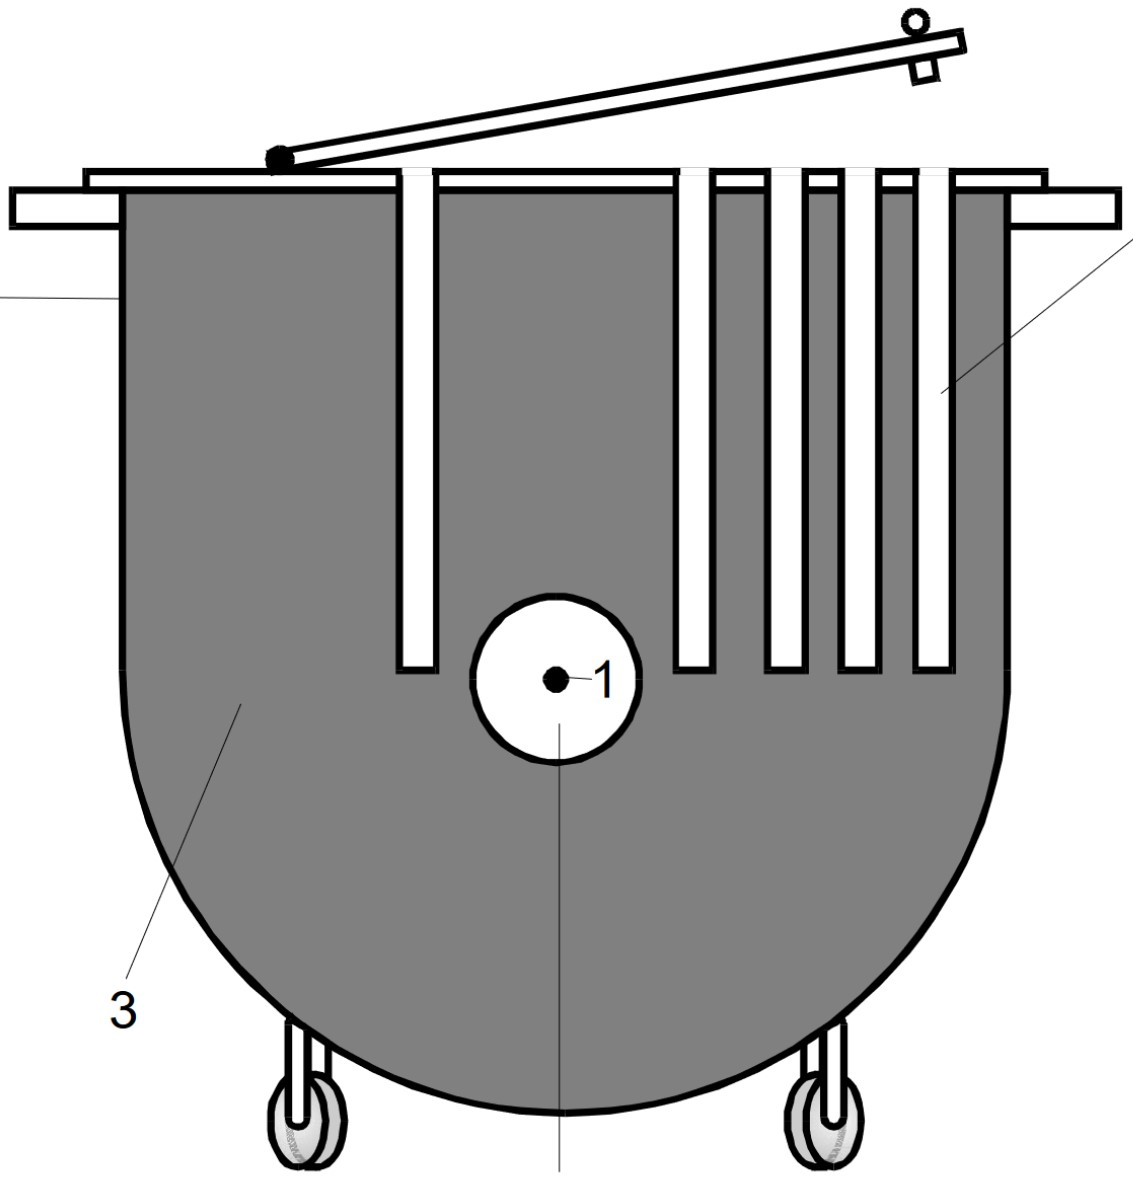
\includegraphics[width=0.5\textwidth]{img/Neutronenquelle.jpg}
    \caption{Schematische Darstellung der Erzeugung thermischer Neutronen. \cite{V702}}
    \label{fig:Neutronenquelle}
\end{figure}

Freie Neutronen sind instabil und müssen deshalb für das Experiment erzeugt werden.
Dies wird durch Beschuss von $\ce{^{9}Be}$-Kernen mit $\alpha$-Teilchen umgesetzt.
\begin{equation*}
    \ce{^{9}_{4}Be} + \ce{^{4}_{2}\alpha} \rightarrow \ce{^{12}_{6}C} + \ce{^{1}_{0}n}
\end{equation*}
Die frei werdenden Neutronen besitzen eine Energie von bis zu $\SI{13.7}{MeV}.$
Ihre Energieverteilung ist kontinuierlich.
Die entstandenen Neutronen diffundieren, wie in \autoref{fig:Neutronenquelle} zu sehen, durch eine Parafinschicht und werden dadurch abgebremst.
Sie geben dabei ihre Energie durch elastische Stöße an die Wasserstoffatome im Parafin ab.
Wasserstoff wird hierbei bevorzugt verwendet, da die bei elastischen Stößen übertragene Energie maximal ist, wenn die Massen der Stoßpartner gleich sind.
Die übertragene Energie kann berechnet werden mit
\begin{equation*}
    E_{\text{ü}} = E_0\frac{4m_{\text{n}}M}{(m_{\text{n}} + M)^2}.
\end{equation*}
Nach dem Durchdringen der Parafinschicht besitzen die Neutronen eine mittlere kinetische Energie von $\SI{0.025}{eV},$
was einer Geschwindigkeit von $\SI{2.2}{\kilo\meter\per\second}$ entspricht.
Diese Neutronen werden thermische Neutronen genannt.
\\
\\
\subsection{Untersuchung des Zerfalls}
\label{subsec:Untersuchung des Zerfalls}

Die untersuchten Isotope gehen durch $\beta^-\,$-Zerfall in ein anderes, stabiles Isotop über.
Radioaktiver Zerfall ist ein statistischer Prozess.
Die Zahl der zu einem bestimmten Zeitpunkt $t$ noch nicht zerfallenen Kerne $N(t)$ werden durch
\begin{equation}\label{eqn:Zerfallsgesetz}
    N(t) = N_0 \textbf{e}^{-\lambda t}
\end{equation}
angegeben. Hierbei ist $N_0$ die Anzahl der bei $t=0$ vorhandenen Kerne des Isotops und $\lambda$ die Zerfallskonstante.	
Die Halbwertszeit $T$ gibt Auskunft darüber, nach welcher Zeit die Hälfte der Kerne zerfallen ist.
Sie ist durch
\begin{equation*}
    \frac{1}{2}N_0 = N_0 \textbf{e}^{-\lambda T}
\end{equation*}
ermittelbar und somit 
\begin{equation*}
    T = \frac{\ln 2}{\lambda}.
\end{equation*}
Es ist schwer die Größe $N(t)$ akkurat zu bestimmen. 
Deshalb wird die Anzahl der in einem Zeitintervall $\Delta t$ zerfallenen Kerne $N_{\Delta t}(t)$ gemessen.
Dabei wird $N_{\Delta t}(t)$ gebildet mit
\begin{equation*}
    N_{\Delta t}(t) = N(t) - N(t + \Delta t),
\end{equation*}
was sich durch Einsetzen von \eqref{eqn:Zerfallsgesetz} zu
\begin{equation*}%Wie sollen hier bitte die verfickten Klammern sitzen?
    \ln N_{\Delta t}(t) = \ln{N_0}\left(1 - \textbf{e}^{-\lambda\Delta t}\right) - \lambda t
\end{equation*}
umformen lässt.
Da $\ln N_0(1 - \textbf{e}^{-\lambda\Delta t})$ konstant ist, kann $\lambda$ durch eine lineare Ausgleichsrechnung bestimmt werden.

\subsubsection{Besonderheit bei Silber}
\label{subsubsec:Besonderheit bei Silber}

In der Natur vorkommendes Silber besteht zu $\SI{52.3}{\percent}$ aus $\ce{^{107}Ag}$ und zu $\SI{48.7}{\percent}$ aus $\ce{^{109}Ag}$.
Beide Isotope sind stabil und können durch Neutroneneinfang yu instabilen Isotope überführt werden.
Der vollständige Prozess im Verlauf des Experiments ist
\begin{equation*}
    \ce{^{107}_{47}Ag} + \ce{^{1}_{0}n} \rightarrow \ce{^{108}_{47}Ag} \rightarrow \ce{^{108}_{48}Cd} + \beta^- + \bar{\nu}_e \label{eqn:Ag107}
\end{equation*}
\begin{equation*}
    \ce{^{109}_{47}Ag} + \ce{^{1}_{0}n} \rightarrow \ce{^{110}_{47}Ag} \rightarrow \ce{^{110}_{48}Cd} + \beta^- + \bar{\nu}_e \label{eqn:Ag109}.    
\end{equation*}
Problematisch ist hierbei, dass sich die Zerfallskurven der beiden Isotope überlagern. 
Da sich die Halbwertszeiten der beiden Isotope stark unterscheiden, können die Zerfallskurven voneinander getrennt werden.
Nach einer hinreichende langen Zeit $t^*$ sind alle kurzlebigeren $\ce{^{110}Ag}$-Kerne zerfallen und es zerfällt nur noch $\ce{^{108}Ag}$.
Durch messen der Zerfälle nach $t^*$ kann die Zerfallskonstante $\lambda_{\text{lang}}$ von $\ce{^{108}Ag}$ bestimmt werden.
Zur bestimmung von $N_{\Delta t, \text{kurz}}$ wird die Anzahl der Zerfälle des langlebigeren Isotops von der Gesamtzahl der Zerfälle abgezogen.
Dies führt zur Gleichung
\begin{equation*}
    N_{\Delta t, \text{kurz}}(t) = N_{\Delta t}(t) - N_{\Delta t, \text{lang}}(t).
\end{equation*} 
Die Zerfallskonstante $\lambda_{\text{kurz}}$ des kurzlebigeren Isotops kann dann durch eine lineare Ausgleichsrechnung bestimmt werden.

\subsection{Nulleffekt}
\label{subsec:Nulleffekt}

Zur Messung der Zerfälle wird ein Geiger-Müller-Zählrohr verwendet.
Es nimmt jedoch neben den Zerfällen auch Umgebungsstrahlung auf. 
Um die Detektion von Umgebungsstrahlung zu minimieren wird das Zählrohr in eine Bleiabschirmung gesteckt.
Es ist dennoch nicht vollständig vermeidbar, dass Umgebungsstrahlung detektiert wird.
Dieser sogenannte Nulleffekt wird vor Beginn der Messung bestimmt und von den Messwerten abgezogen.
\newpage